\documentclass[compress]{beamer}
\setbeamertemplate{section in toc}[sections numbered]
\usepackage{dl2016}
\usepackage{verbatim}
\usepackage{algorithmic}
\usepackage{mathtools}
\usepackage{xcolor, graphicx}
\graphicspath{{./figures/}}


\author{
   \textbf{Thomas Hofmann} \\[5mm] 
   { \footnotesize Institute for Machine Learning \\ ETH Zurich }
\vspace*{-10mm}
} 
\def\imagetop#1{\vtop{\null\hbox{#1}}}
\def\is#1{\setlength{\itemsep}{#1}}
\renewcommand{\vec}[1]{{\mathbf #1}}
\newcommand{\sphere}[1]{{\mathcal S^{#1}}}
\renewcommand{\x}{{\vec x}}
\newcommand{\h}{{\vec h}}
\newcommand{\D}{{\mathcal D}}
\newcommand{\V}{{\mathcal V}}
\renewcommand{\w}[1]{w^{#1}}
\newcommand{\z}{{\vec z}}
\newcommand{\y}{{\vec y}}

\title{{\Large \textbf{Deep Learning for \\Natural Language Understanding}}}

\date{October 20, 2016}

\begin{document}

\frame[plain]{\titlepage}

%%%%%%%%%%
\begin{frame}
\frametitle{Overview} 
\tableofcontents
\end{frame}

\section{
%%%%%%%%%%%%%%%%%%%%
%%%%%%%%%%%%%%%%%%%%
Language as a Scientific Frontier
%%%%%%%%%%%%%%%%%%%%
%%%%%%%%%%%%%%%%%%%%
}
\frame{\sectionpage}

%%%%%%%%%%
\begin{frame}
\frametitle{
%%%%%%%%%%
Natural Language Understanding
%%%%%%%%%%
}

\vspace*{-4mm}
\begin{flushright}
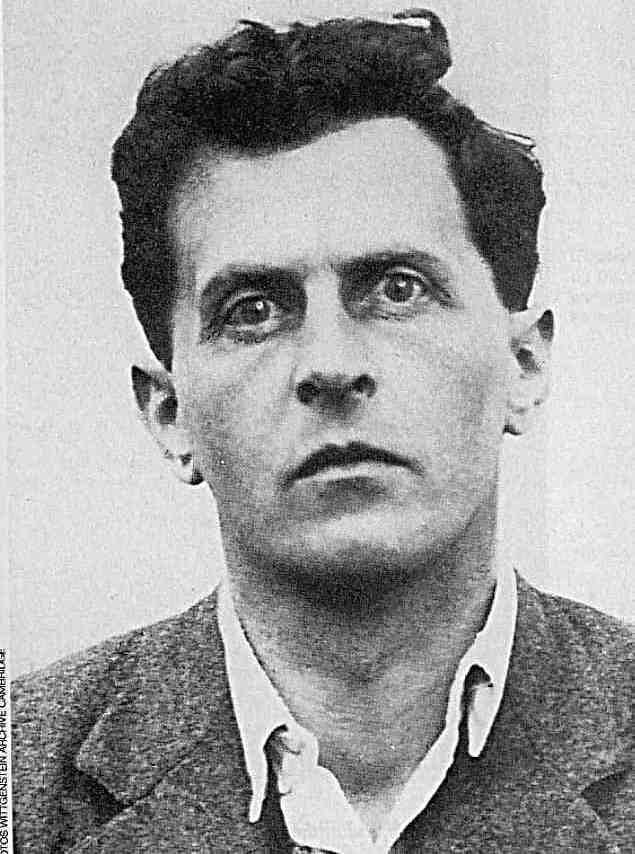
\includegraphics[width=21mm]{wittgenstein}
\end{flushright}
\vspace*{-10mm}

The Opportunity:\\[4mm]
\textit{The meaning of a word is its use in language.}\\[1mm]
(Wittgenstein, Philosophical Investigations �43, 1953)\\[5mm]

Gigantic digital corpus of actual usage of language available \\[1mm]
$\Longrightarrow$ should be able to learn statistical models of meaning from data
\end{frame}

%%%%%%%%%%
\begin{frame}
\frametitle{
%%%%%%%%%%
Natural Language Understanding
%%%%%%%%%%
}

\vspace*{-4mm}
\begin{flushright}
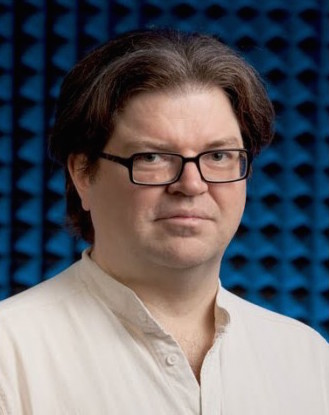
\includegraphics[width=21mm]{lecun}
\end{flushright}
\vspace*{-10mm}

The Impact:\\[4mm]
\textit{Natural Language Processing is the next frontier in AI}\\[1mm]
(Yann LeCun, Facebook AI Research, 2015)\\[5mm]

Machines that understand language = true scientific revolution \\[1mm]
$\Longrightarrow$ knowledge processing, human-computer interfaces, social interactions, thinking machines (!?)
\end{frame}

%%%%%%%%%%
\begin{frame}
\frametitle{
%%%%%%%%%%
Natural Language Understanding
%%%%%%%%%%
}

\vspace*{-4mm}
\begin{flushright}
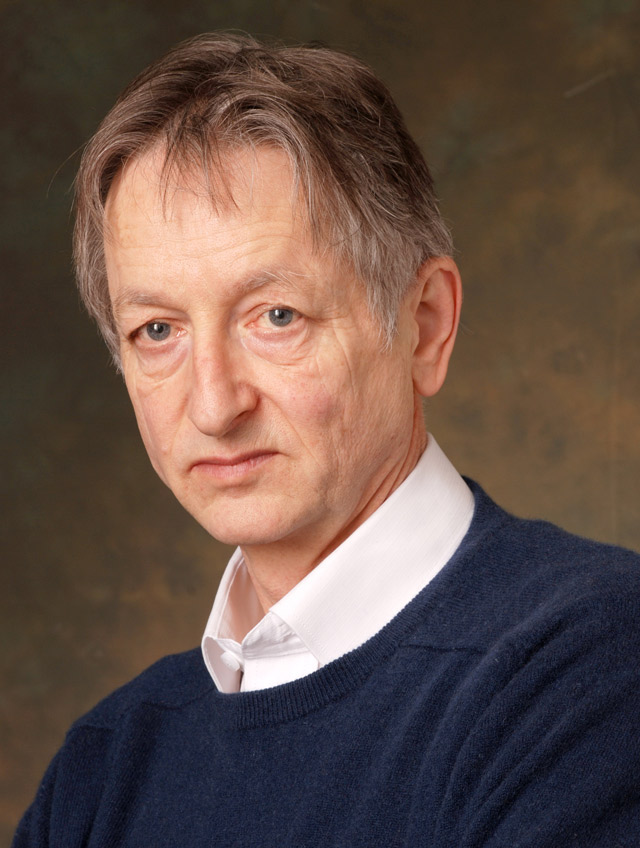
\includegraphics[width=21mm]{hinton}
\end{flushright}
\vspace*{-10mm}

The Approach:\\[4mm]
Deep networks provide a new "architectural toolbox" to design and learn models for natural language understanding.
\\[5mm]

Large reportoire of methods: embeddings, convolutional layers, recurrent and recursive models, gated units, attention networks \\[1mm]
$\Longrightarrow$ moved the needle on many NLU problems, but: how far will it advance machine intelligence?
\end{frame}


\section{
%%%%%%%%%%%%%%%%%%%%
%%%%%%%%%%%%%%%%%%%%
Words
%%%%%%%%%%%%%%%%%%%%
%%%%%%%%%%%%%%%%%%%%
}
\frame{\sectionpage}


%%%%%%%%%%
\begin{frame}
\frametitle{
%%%%%%%%%%
Symbolic Units
%%%%%%%%%%
}
\underline{Fundamental Problem}: language is composed of \textblue{symbols} (e.g.~characters, words)
\begin{itemize}
\is{2mm}
\item no "signals" or continuous measurements  (vs.~vision, speech)
\item connection between phones/morphems and meaning largely based on convention 
\item conventions are expressed in repeated usage of words\\(i.e.~symbols can be re-identified, but are otherwise arbitrary) 
\item language usage = utterance (pragmatic dimension)
\end{itemize}
\end{frame}

%%%%%%%%%%
\begin{frame}
\frametitle{
%%%%%%%%%%
Word Embeddings 
%%%%%%%%%%
}
\underline{Basic idea}: map symbols to vector representation = \textred{embedding} into a (Euclidian) vector space
\begin{align*}
\text{symbolic} \quad \mathcal V \ni w \; \stackrel{\text{embed}}\mapsto \; \x_w \in \Re^d \quad \text{quantitative} 
\end{align*}

Interpret vectors as latent variables and link them to observable through a probabilistic model.\\[4mm]

\underline{Simplest case}: pairwise \textred{word co-occurrence}
\begin{align*}
\text{pmi}(v,w) = \log \frac{p(v,w)}{p(v) p(w)} = \log\frac{p(v|w)}{p(v)} =  \x_v^\top \x_w + \text{const}
% -\log p(v) 
\end{align*}
\vspace*{-4mm}
\begin{itemize}
\is{1mm}
\item pointwise mutual information related to inner product between latent vectors % (marginals modeled seperately)
\end{itemize}
\end{frame}


%%%%%%%%%%
\begin{frame}
\frametitle{
%%%%%%%%%%
Skip-gram Model 
%%%%%%%%%%
}
Pairwise occurrences of words in \textblue{context window} (of fixed size $R$)\\[3mm]

Simplified: text = long sequence of words, $\mathbf w = (w_1,\dots,w_T)$.\\[0.5mm]
Co-occurrence index set $\mathcal C_R := \{ (i,j): 1 \le |i-j| \le R\}$. \\[4mm]

\textblue{Skip-gram} objective (Mikolov et al, 2013): 
\begin{align*}
\mathcal{L}(\theta) = 
\sum_{(i,j) \in \mathcal C_R} 
\log\left[ \frac{p_\theta(w_i|w_j)}{p(w_i)} \right] + 
\log\left[ \frac{p_\theta(w_j|w_i)}{p(w_j)} \right] 
\end{align*}
\vspace*{-4mm}
\begin{itemize}
\item model conditionals, ignore marginals (computational plus)
\item two vectors per word (allow for asymmetry), $\theta = (\x_w,\z_w)_{w \in \V}$
\begin{align*}
\log p_\theta(v|w) = \x_v^\top \z_w - \log \sum_{u \in \V} \exp\left[ \x_{u}^\top \z_w \right]
\end{align*}
\end{itemize}

\end{frame}

%%%%%%%%%%
\begin{frame}
\frametitle{
%%%%%%%%%%
Skip-Gram Model 
%%%%%%%%%%
}

\vspace*{4mm}
Computational aspects:
\vspace*{-2mm}
\begin{itemize}
\item expensive to compute log-partition function (sum over $\V$)
\item trick \#1: use negative sampling (importance sampling)
\item trick \#2: subsample frequent words 
\item can be trained with corpora w/ Bs of words
\end{itemize}

Results: semantic analogies captured by word embeddings\\[1mm]
\begin{center}
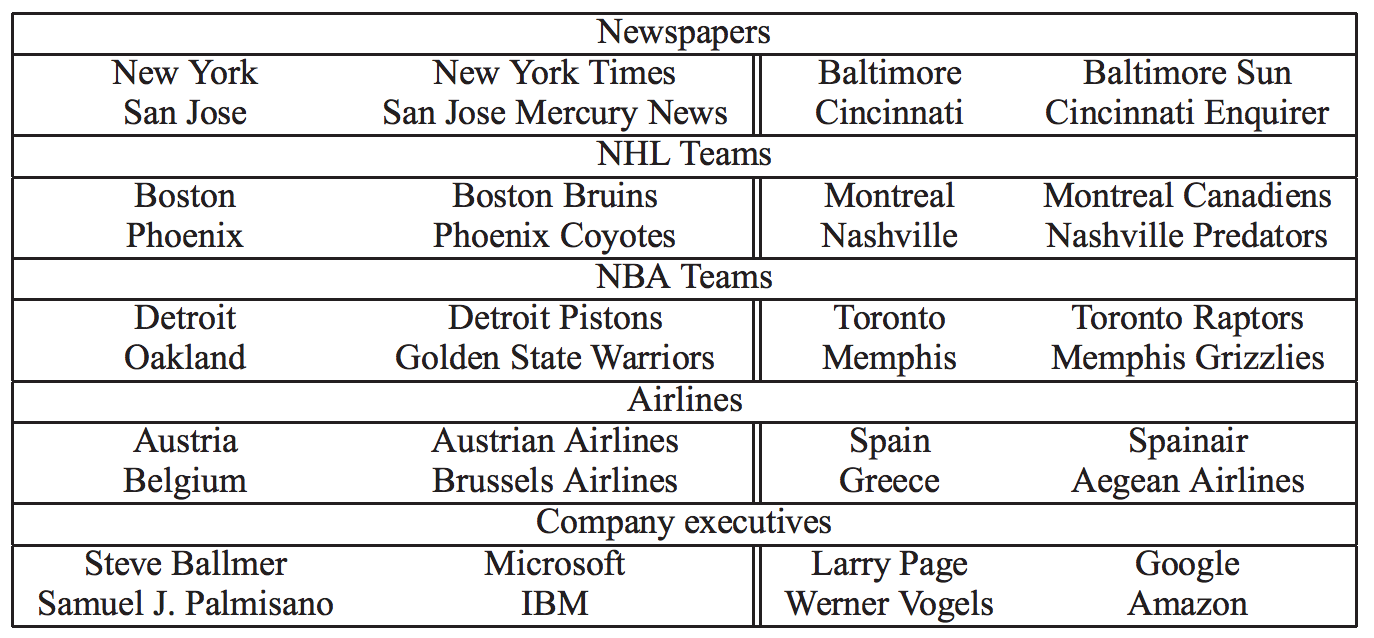
\includegraphics[width=0.7\textwidth]{analogy}
\end{center}

\end{frame}

%%%%%%%%%%
\begin{frame}
\frametitle{
%%%%%%%%%%
Discussion
%%%%%%%%%%
}

Word embeddings have become a standard tool in natural language understanding and information retrieval within less than 2 years.\\[4mm]

Simple, but essential step in moving from symbols to vectors. \\[4mm]

Many variants, e.g. GloVe (Pennington, Socher \&  Manning, 2014), embeddings as matrix factorization (Levy \& Goldberg, 2014)\\[4mm]

Code and pre-trained embeddings.\\
\url{code.google.com/archive/p/word2vec}



\end{frame}


\section{
%%%%%%%%%%%%%%%%%%%%
%%%%%%%%%%%%%%%%%%%%
Word Sequences 
%%%%%%%%%%%%%%%%%%%%
%%%%%%%%%%%%%%%%%%%%
}
\frame{\sectionpage}


%%%%%%%%%%
\begin{frame}
\frametitle{
%%%%%%%%%%
From Words to Sequences of Words 
%%%%%%%%%%
}

\underline{Question}: Can we extend word embeddings to embeddings for \textblue{sequences of words}? \\[6mm]

Why is this relevant? Fundamental question of \textblue{statistical language modeling} (cf.~Shannon).
\begin{align*}
\text{estimate} \; \; p(w_1 \dots w_T) = \prod_{t=1}^T p(w_t | w_{t-1} \dots w_{1})
\end{align*}
\vspace{-5mm}
\begin{itemize}
\is{2mm}
\item predict next word in a sequence of words
\item quality measured by perplexity (exp of average log-probability)
\end{itemize}

\end{frame}

%%%%%%%%%%
\begin{frame}
\frametitle{
%%%%%%%%%%
From Words to Sequences of Words 
%%%%%%%%%%
}


\textblue{Traditional approach}: $k$-th order Markov assumption 
\begin{align*}
p(w_t | w_{t-1} \dots w_{1}) \approx p(w_t | w_{t-1} \dots w_{t-k}) \approx \text{$(k+1)$-gram counts}
\end{align*}
\vspace*{-8mm}
\begin{itemize}
\item in practice: $5$-grams, i.e.~$k=4$
\item advanced smoothing techniques (Kneser-Ney smoothing)
\end{itemize}
\vspace*{5mm}

\textred{Modern approach}: language models via embeddings
\begin{align*}
\log p(v | \mathbf w := w_1, \dots w_{t-1}) = \x_v^\top \z_{\mathbf w} + \text{const} 
\end{align*}
\vspace*{-8mm}
\begin{itemize}
\item  $\x_v = $ word embedding 
\item  $\z_{\mathbf w} = $ sequence embedding 
\item \underline{Question}: how can we construct sequence embeddings?
\end{itemize}
\end{frame}


%%%%%%%%%%
\begin{frame}
\frametitle{
%%%%%%%%%%
From Words to Sequences of Words 
%%%%%%%%%%
}

Three main approaches:\\[5mm]

1.~\textblue{Convolutional networks}\\[1mm]
\begin{itemize}
\is{1mm}
\item pros: conceptually simple, fast to train
\item cons: limited range memory
\end{itemize}
\vspace*{2mm}

2.~\textblue{Recurrent networks}\\[1mm]
\begin{itemize}
\is{1mm}
\item pros: active memory management via gated units 
\item cons: more difficult to optimize, larger data sets needed
\end{itemize}
\vspace*{2mm}
 
 3.~\textblue{Recursive networks} (in combination with parsers)
 

\end{frame}




%%%%%%%%%%
\begin{frame}
\frametitle{
%%%%%%%%%%
ConvNets: Word Representations
%%%%%%%%%%
}
\underline{Idea}: use convolutional network on top of word embeddings \\-- take a deep learning view!\\[9mm]

\begin{columns}
\begin{column}{0.45\textwidth} 
Step 1: map word sequence to vector sequence
\end{column} 
\begin{column}{0.45\textwidth} 
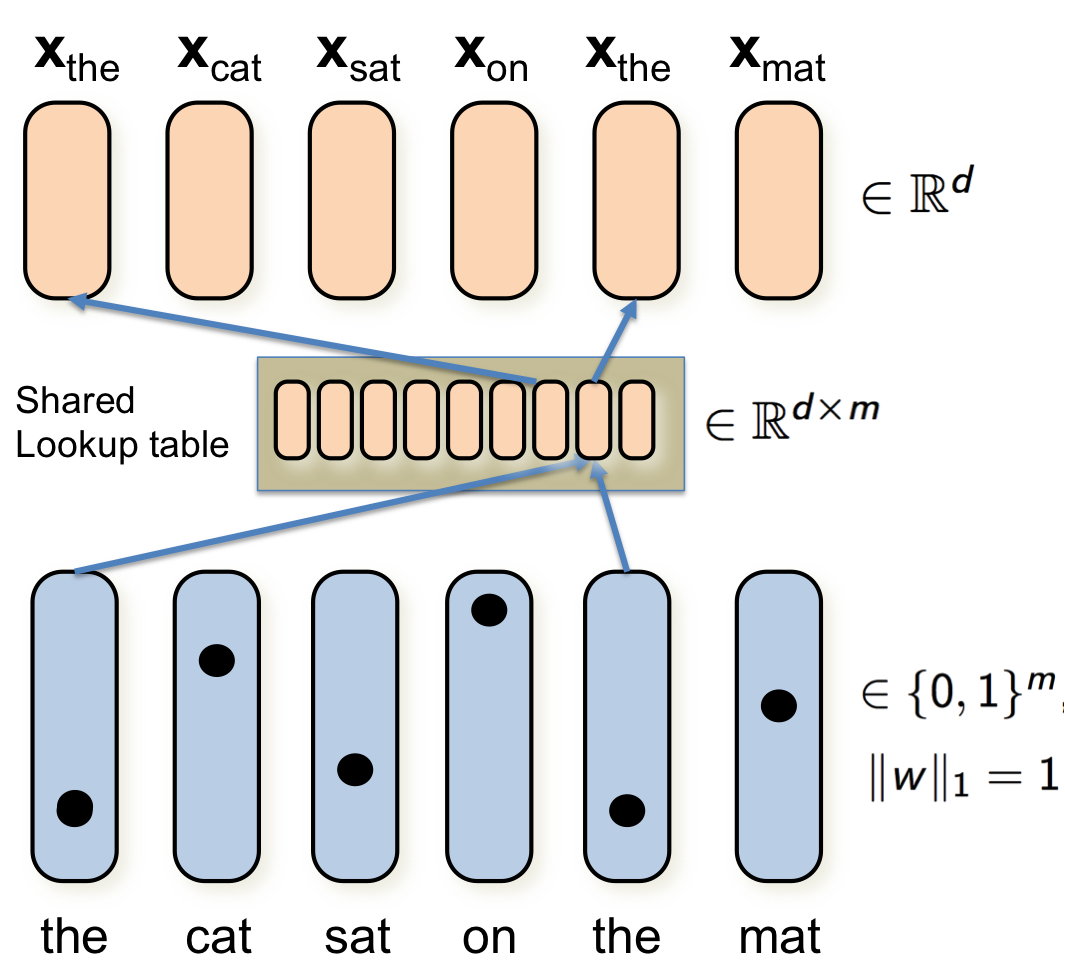
\includegraphics[width=1\textwidth]{embed.png}
\end{column} 
\end{columns}
\end{frame}

%%%%%%%%%%
\begin{frame}
\frametitle{
%%%%%%%%%%
ConvNets: Concatenation
%%%%%%%%%%
}

\begin{columns}
\begin{column}{0.45\textwidth} 
Step 2: concatenate vectors \\[1mm] (variable length)
\end{column} 
\begin{column}{0.45\textwidth} 
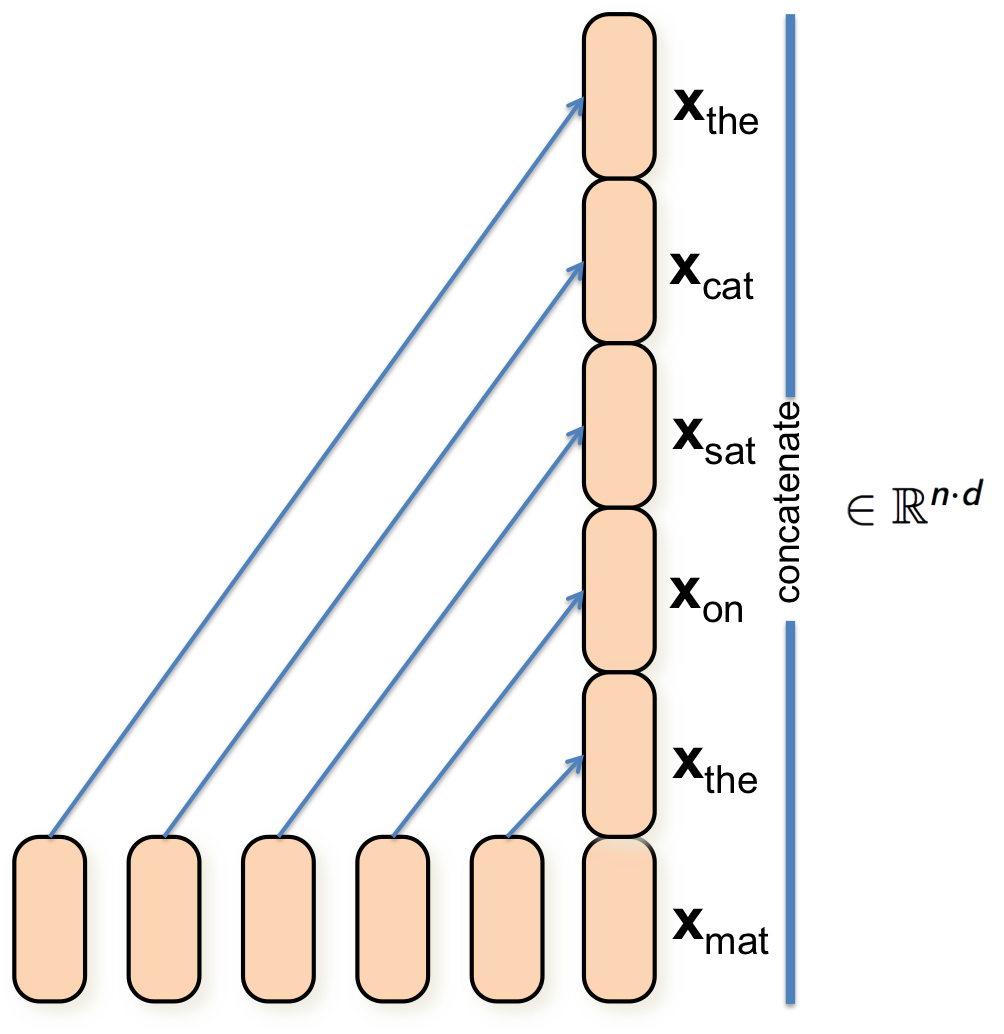
\includegraphics[width=1\textwidth]{embedseq.png}
\end{column} 
\end{columns}
\end{frame}


%%%%%%%%%%
\begin{frame}
\frametitle{
%%%%%%%%%%
ConvNets: Channels
%%%%%%%%%%
}

\begin{columns}
\begin{column}{0.55\textwidth} 
Step 3: convolve \\[4mm]

chose window size(s), e.g.~$3$ or $5$\\[4mm]

single channel $f_j: \Re^{3d} \to \Re$\\[1mm]
\begin{itemize}
\is{1mm}
\item shift mask over input
\item parameter sharing (filters)
\item nonlinearity (tanh or ReLU)
\end{itemize}
\vspace*{4mm}

$k$ independent channels 
%\\[1mm]
%\begin{itemize}
%\is{1mm}
%\item padding: compute $n \cdot k$ numbers
%\item = hidden layer activities
%\end{itemize}
\end{column} 

\begin{column}{0.4\textwidth} 
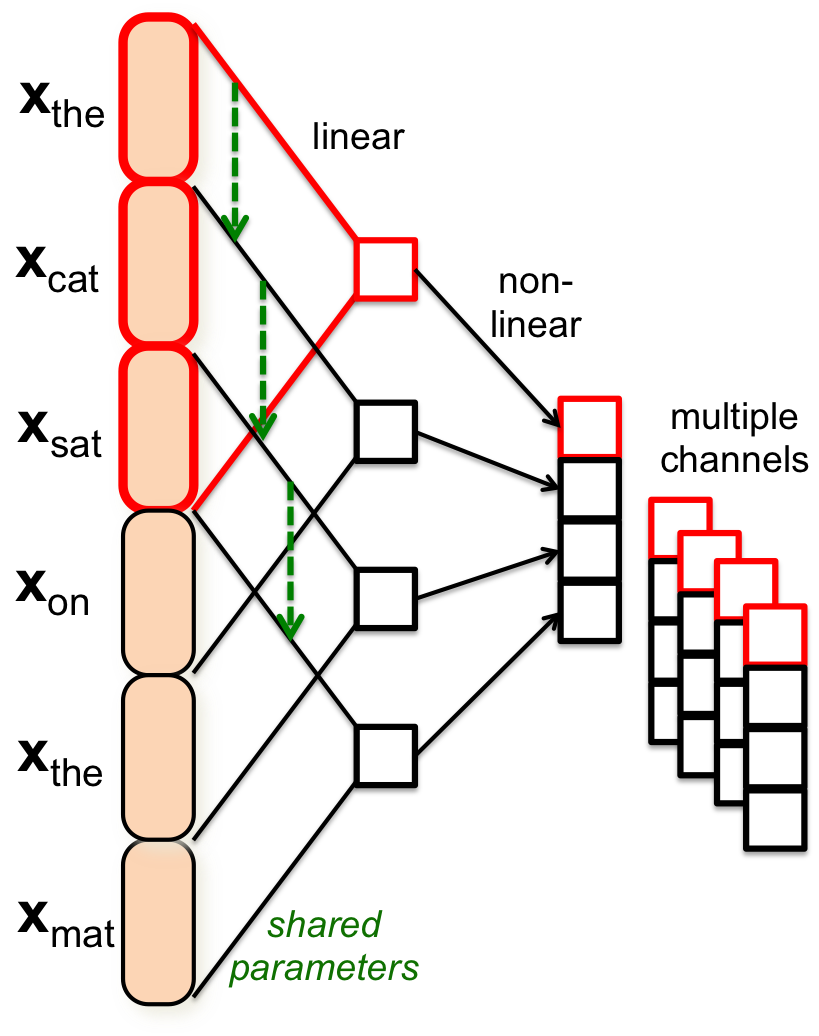
\includegraphics[width=1\textwidth]{convolution.png}
\end{column} 
\end{columns}
\end{frame}


%%%%%%%%%%
\begin{frame}
\frametitle{
%%%%%%%%%%
ConvNets: Pooling
%%%%%%%%%%
}

\begin{columns}
\begin{column}{0.55\textwidth} 
Step 4: pooling \\[3mm]
reduce each channel (variable length) to single number\\[2mm]
\begin{itemize} 
\is{3mm}
\item mathematically: $\Re^{n \times k} \to \Re^k$
\item typically: \textblue{max-over-time} pooling  (no parameters)
\item map word sequence to fixed-length representation
\end{itemize}
\end{column} 
\begin{column}{0.4\textwidth} 
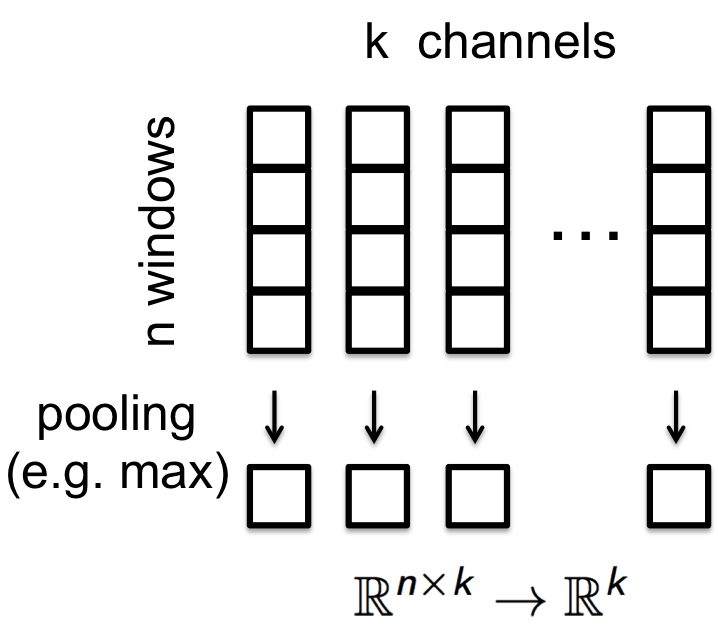
\includegraphics[width=1\textwidth]{pooling}
\end{column} 
\end{columns}

\end{frame}

%%%%%%%%%%
\begin{frame}
\frametitle{
%%%%%%%%%%
ConvNets: Softmax
%%%%%%%%%%
}

\begin{columns}
\begin{column}{0.55\textwidth} 
Step 5: SoftMax \\[4mm]

predict words via soft-max\\[2mm]
\begin{align*}
p(v | \vec w) = \frac{\exp \left[ \langle \y_v, \z_{\vec w} \rangle \right]}{ \sum_{u \in \V} \exp \left[ \langle \y_{u}, \z_{\vec w} \rangle\right]}
\end{align*}
\begin{itemize} 
\is{2mm}
\item uses word embeddings  $\y_v \in \Re^k$ 
\item two types of word embeddings ($\x_v \in \Re^d$, $\y_v \in \Re^k$)
\end{itemize}\end{column} 
\begin{column}{0.4\textwidth} 
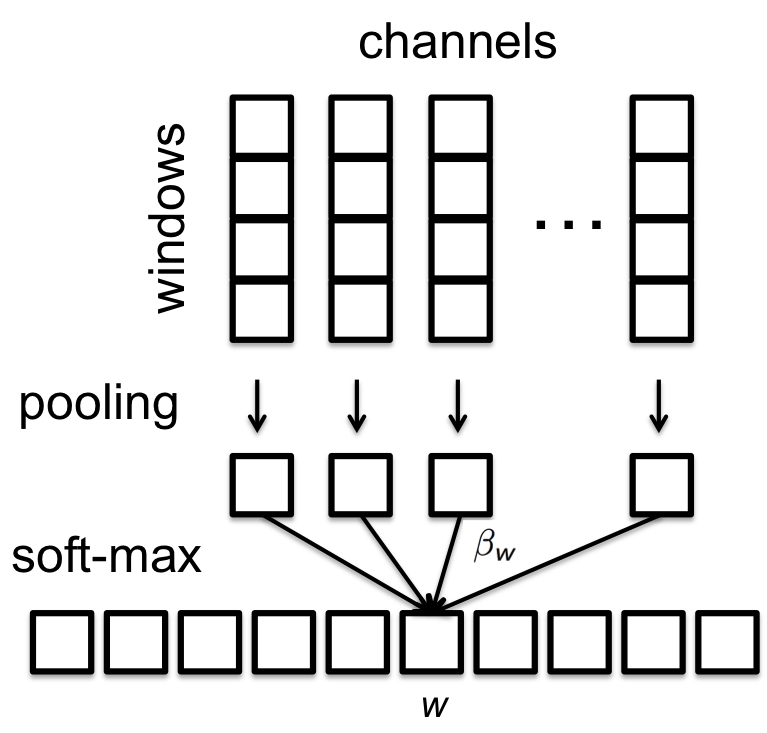
\includegraphics[width=1\textwidth]{softmax}
\end{column} 
\end{columns}
\end{frame}

%%%%%%%%%%
\begin{frame}
\frametitle{
%%%%%%%%%%
ConvNets: Applications
%%%%%%%%%%
}

ConvNet architecture was used in early neural language models.\\
(Bengio et al, 2003; Bengio et al, 2006 )\\[4mm]

Can be extended to character level models (no word segmentation).\\[4mm]

Useful architecture for supervised tasks -- example: \textblue{sentiment prediction} for blogs. 
\begin{itemize}
\item replace softmax layer over vocabulary by softmax over classes
\end{itemize}
\vspace*{4mm}

Models typically trained in an end-to-end fashion. 

\end{frame}

%%%%%%%%%%
\begin{frame}
\frametitle{
%%%%%%%%%%
Sentiment Classification
%%%%%%%%%%
}

Automatically classify sentiment in tweets (= short piece of text). \\[1mm]
Ternary classification: positive, neutral, negative.\\[5mm]

\begin{columns}
\begin{column}{0.5\textwidth}
SemEval 2016 competition \\[1mm]
(Jan Deriu,  Maurice Gonzenbach, Martin Jaggi, Aurelien Lucchi) 
\begin{itemize}
\is{2mm}
\item two-stage ConvNet
\item data augmentation: 4.3M $\to$ 90M (emoticons)
\item pre-training (distant supervision) 
\end{itemize}
\end{column}
\begin{column}{0.4\textwidth}
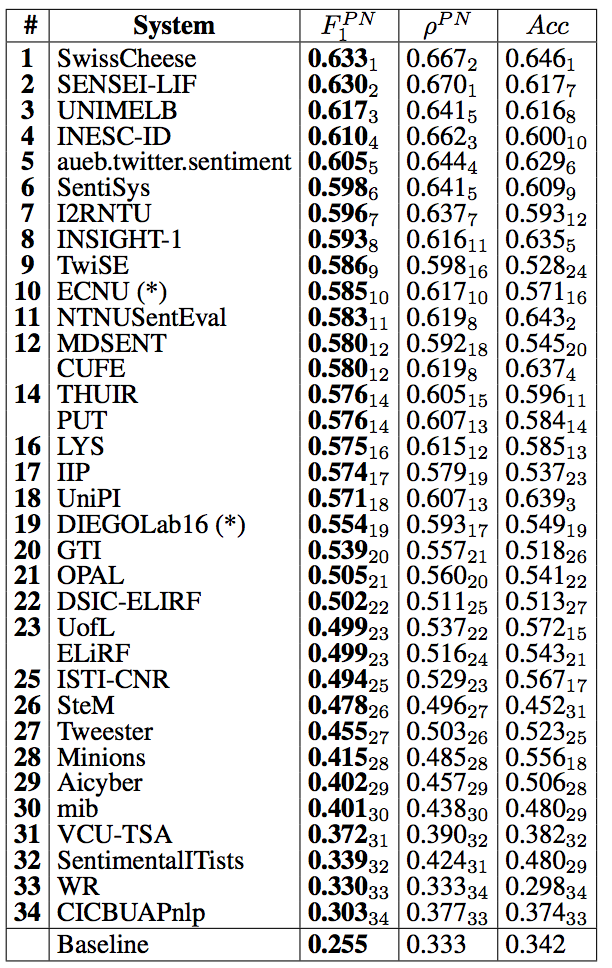
\includegraphics[width=0.84\textwidth]{cheese}
\end{column}
\end{columns}

\end{frame}

\section{
%%%%%%%%%%%%%%%%%%%%
%%%%%%%%%%%%%%%%%%%%
Gated Units and Memory
%%%%%%%%%%%%%%%%%%%%
%%%%%%%%%%%%%%%%%%%%
}
\frame{\sectionpage}



%%%%%%%%%%
\begin{frame}
\frametitle{
%%%%%%%%%%
Recurrent Networks 
%%%%%%%%%%
}

Basic Idea: evolve a fixed dimensional hidden state sequence over time (cf.~Kalman filtering) = \textblue{memory}
\begin{align*}
& (w_1,\dots,w_t) \mapsto (\h_{1}, \dots,\h_t) , \quad \text{where} \;\; \h_{t} = F(\h_{t-1},w_t)
\end{align*}
\vspace*{-6mm}
\begin{itemize}
\item natural generalization of word embeddings, $\h_t = \x_{w_t}$
\end{itemize}
\vspace*{3mm}

Simplest model: recurrent network (rolled out feedforward network)
\begin{align*}
F(\h,w) = \sigma\left( \mathbf U \h + \mathbf W \x_{w} \right), \quad \text{$\sigma$: pointwise non-linearity}
\end{align*}
\vspace*{-6mm}
\begin{itemize}
\item challenge: instable (vanishing/exploding) gradients 
\item heuristics: use $\sigma =$ rectified linear units; gradient clipping  
\end{itemize}
 \end{frame}



%%%%%%%%%%
\begin{frame}
\frametitle{
%%%%%%%%%%
Gated Units
%%%%%%%%%%
}

Basic idea: better capture long-term dependencies via \textblue{explicit management of persistent memory}\\[1mm]
\begin{itemize}
\is{3mm}
\item use gated units to evolve memory
\item gates: multiplicative gain control 
\item standard version: long-short-term memory (LSTM) units 
\end{itemize}

Diagrammtic view (next slide) 
\end{frame}

%%%%%%%%%%
\begin{frame}
\frametitle{
%%%%%%%%%%
Gated Units
%%%%%%%%%%
}

\begin{center}
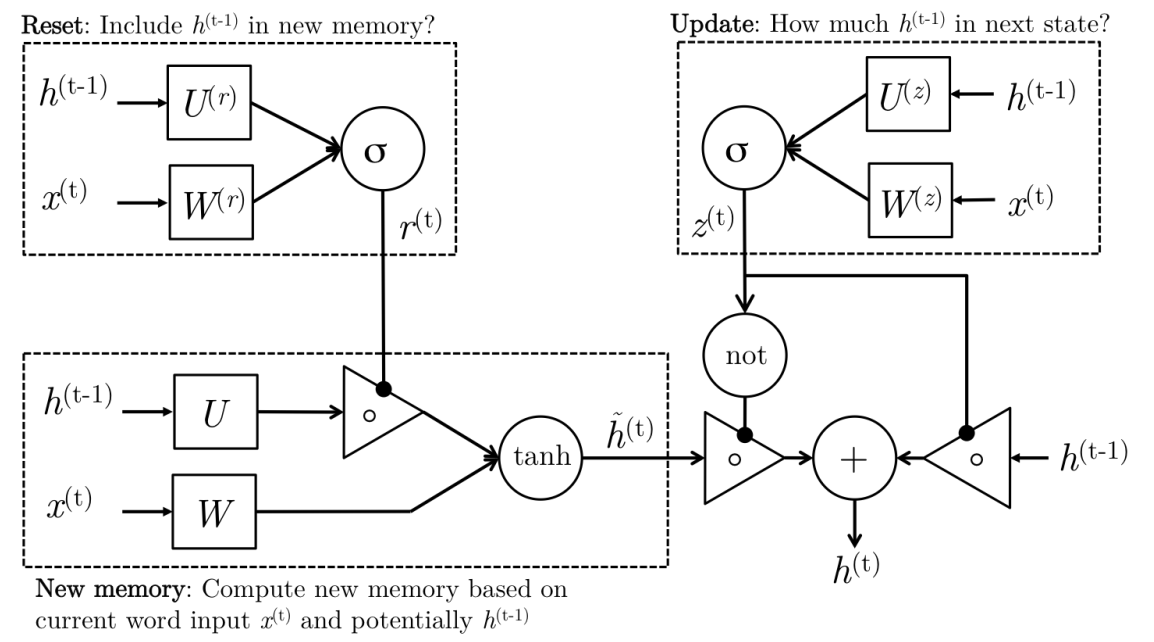
\includegraphics[width=0.89\textwidth]{gru}\\
{\footnotesize (c) Richard Socher}
\end{center}

\end{frame}

%%%%%%%%%%
\begin{frame}
\frametitle{
%%%%%%%%%%
Deep RNNs
%%%%%%%%%%
}

\begin{columns}
\begin{column}{0.5\textwidth}
Idea: stack multiple layers of hidden units on top of each other\\
\begin{itemize}
\is{2mm}
\item replace word embeddings by previous lower level hidden vector 
\item each layer evolves as before (using gated units) 
\end{itemize}
\end{column}
\begin{column}{0.4\textwidth}
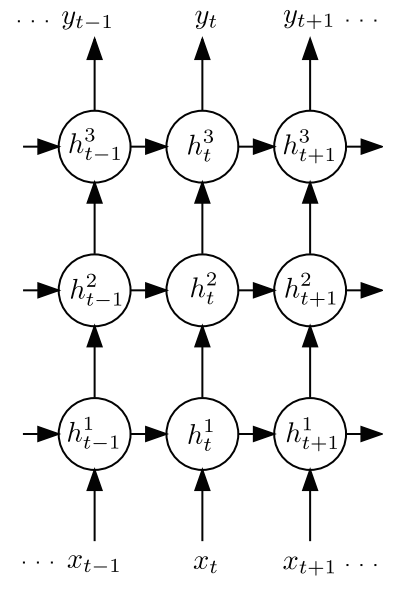
\includegraphics[width=\textwidth]{deeprnn}
\end{column}
\end{columns}

\end{frame}

%%%%%%%%%%
\begin{frame}
\frametitle{
%%%%%%%%%%
Reducing  Model Dimensionality 
%%%%%%%%%%
}

Idea: use linear projections in state evolution \\[2mm]
\begin{align*}
F(\h,w) = \sigma\left( \mathbf U \mathbf V \h + \mathbf W \x_{w} \right), \quad \mathbf U \in \Re^{d \times r}, \mathbf V \in \Re^{r \times d}
\end{align*}
\begin{itemize}
\is{2mm}
\item reduce size of models (as $\h_t \in \Re^d$, $d \approx 10000$)
\item relevant for complexity control, but also with regard to GPU memory limitations
\end{itemize}

\end{frame}



%%%%%%%%%%
\begin{frame}
\frametitle{
%%%%%%%%%%
Language Modeling
%%%%%%%%%%
}

\begin{center}
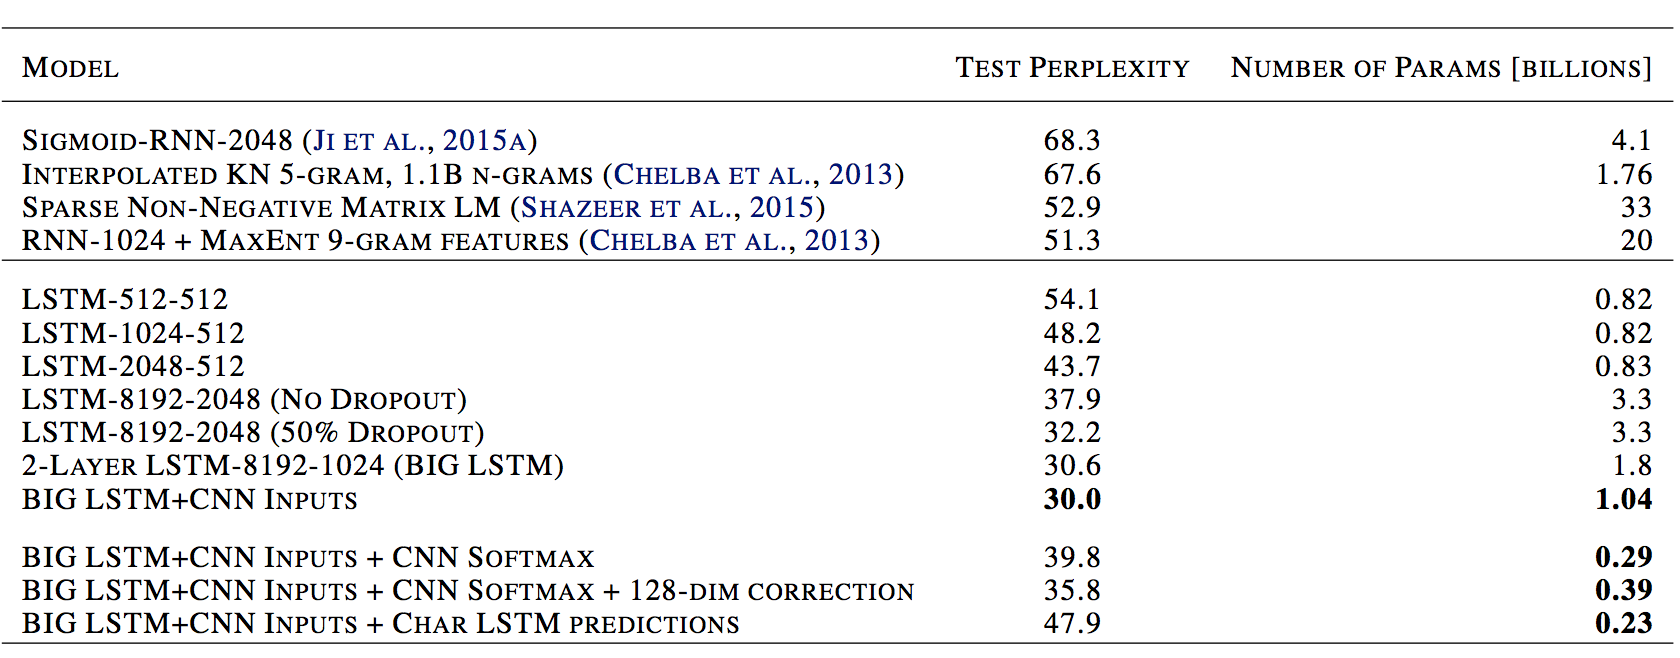
\includegraphics[width=1\textwidth]{biglm}\\
{\footnotesize from Jozefowicz et al, 2016}
\end{center}
\vspace*{-4mm}
\begin{itemize}
\is{2mm}
\item evaluation on corpus w/ 1B words
\item number of parameters can be in the 100Ms or even Bs!
\item ensembles can reduce perplexity to $\approx 23$ (best result 06/2016)
\end{itemize}
\end{frame}

\section{
%%%%%%%%%%%%%%%%%%%%
%%%%%%%%%%%%%%%%%%%%
Sequence-to-Sequence Models
%%%%%%%%%%%%%%%%%%%%
%%%%%%%%%%%%%%%%%%%%
}
\frame{\sectionpage}

%%%%%%%%%%
\begin{frame}
\frametitle{
%%%%%%%%%%
Sequence-to-Sequence Learning
%%%%%%%%%%
}

\underline{Goal}: map sequence of words to new sequence of words
\begin{align*}
\mathbf v = (v_1,\dots,v_t)  \mapsto (w_1,\dots,w_s) = \mathbf w
\end{align*}
\vspace*{-4mm}
\begin{itemize}
\is{2mm}
\item use case: \textblue{machine translation}, translate sentence in one language to sentence in other language 
\item autoencoding to learn sentence embeddings \\(Hinton: \textred{thought vectors})
\end{itemize}

\end{frame}


%%%%%%%%%%
\begin{frame}
\frametitle{
%%%%%%%%%%
Bidirectional Recurrent Networks 
%%%%%%%%%%
}

\begin{columns}
\begin{column}{0.5\textwidth}
Make network bi-directional\\ (Schuster \& Paliwal, 1997)\\[3mm]
Sequence can be process left-to-right or right-to-left\\[3mm]
Combine both approaches (hacky!)
\end{column}
\begin{column}{0.4\textwidth}
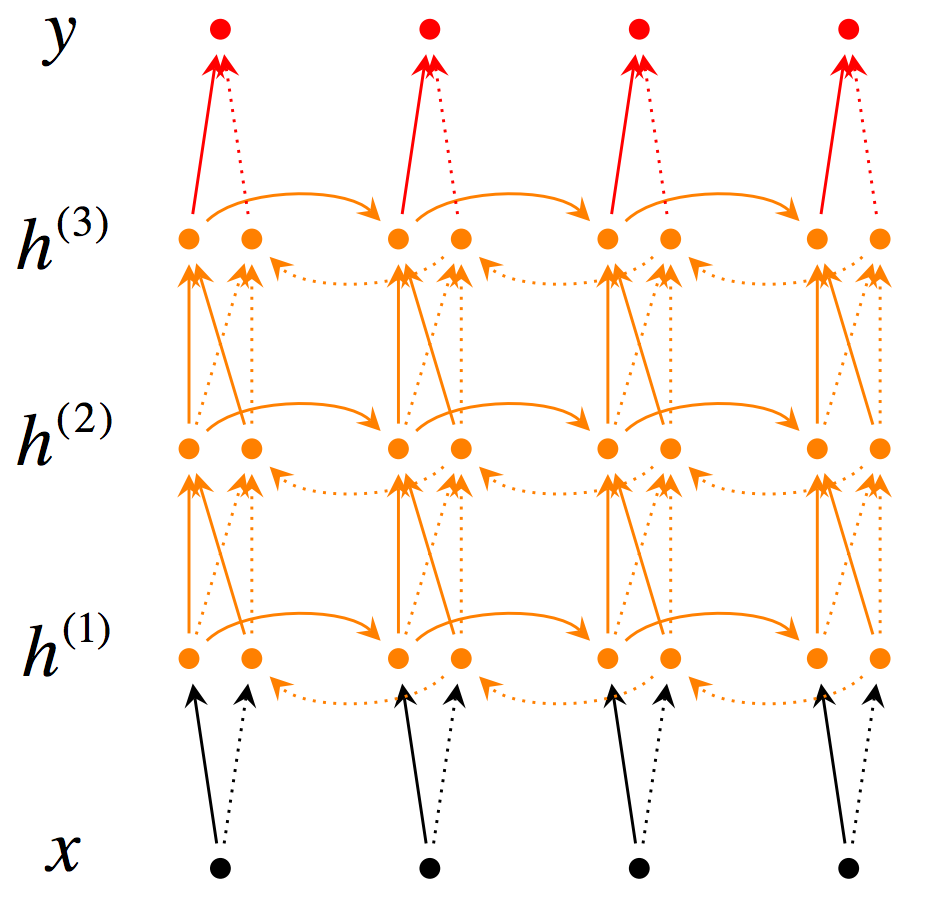
\includegraphics[width=1.0\textwidth]{bideep} \\
\begin{center}
\footnotesize (c) R. Socher  2015
\end{center}
\end{column}
\end{columns}


\end{frame}

%%%%%%%%%%
\begin{frame}
\frametitle{
%%%%%%%%%%
Sequence-to-Sequence Learning
%%%%%%%%%%
}

\textblue{Encode}  source sequence $\mathbf v = (v_1,\dots, v_t)$ into $\z_{\mathbf v} \in \Re^d$. \\[3mm]

\textred{Decode} into target sequence $\vec w$. How can this be done? \\[5mm]

Use same GRU model: generated words are fed back as input\\
(Sutskever, Vinyals, Le, NIPS 2014)
\begin{align*}
p(v | \vec w) \propto \exp\left[ \y_v^\top \vec h_{\vec w} \right], \quad  h_{w_1,\dots,w_t} = \text{GRU}(h_{w_1,\dots w_{t-1}}, w_{t})
\end{align*}

\begin{center}
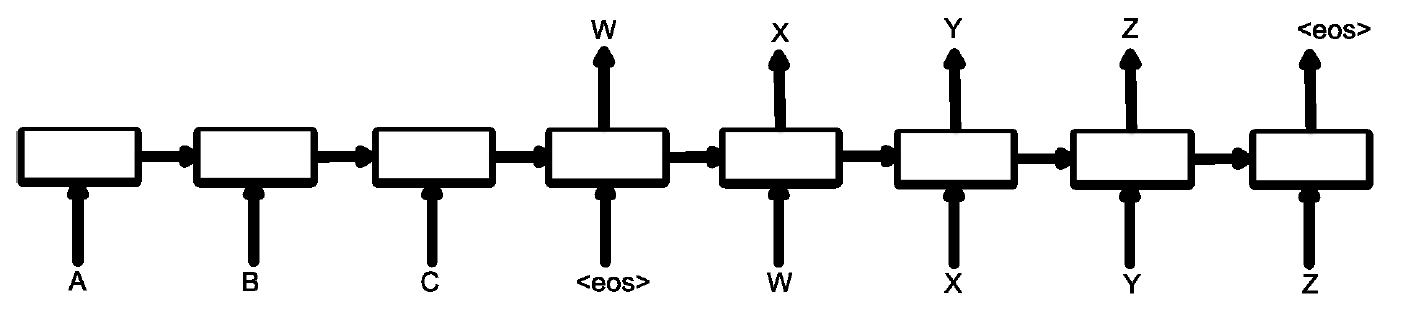
\includegraphics[width=0.7\textwidth]{seq2seq}
\end{center}

\end{frame}

%%%%%%%%%%
\begin{frame}
\frametitle{
%%%%%%%%%%
Machine Translation
%%%%%%%%%%
}

Use seq2seq approach for \textblue{machine translation}.\\[1mm]
(Bahdanau, Cho, Bengio, 2015) \\[4mm]

Encoder: bi-directional RNN (e.g.~w/ GRUs)\\[1mm]
Decoder: RNN with alignment model (\textit{beyond scope})\\[5mm]


Many variants: e.g.~using attention mechanism.\\[1mm]
Current status: deep learning models matching state-of-the-art, perhaps slightly better  

%\begin{columns}
%\begin{column}{0.45\textwidth}
%Results (on WMT'14 corpus)
%\end{column}
%\begin{column}{0.45\textwidth}
%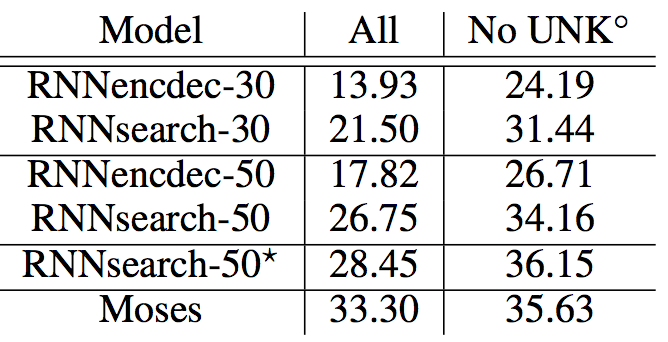
\includegraphics[width=\textwidth]{blue}
%\end{column}
%\end{columns}
\end{frame}

%%%%%%%%%%
\begin{frame}
\frametitle{
%%%%%%%%%%
Multilanguage MT  w/ Character Models
%%%%%%%%%%
}

Lee, Cho \& Hofmann, 2016\\[1mm]
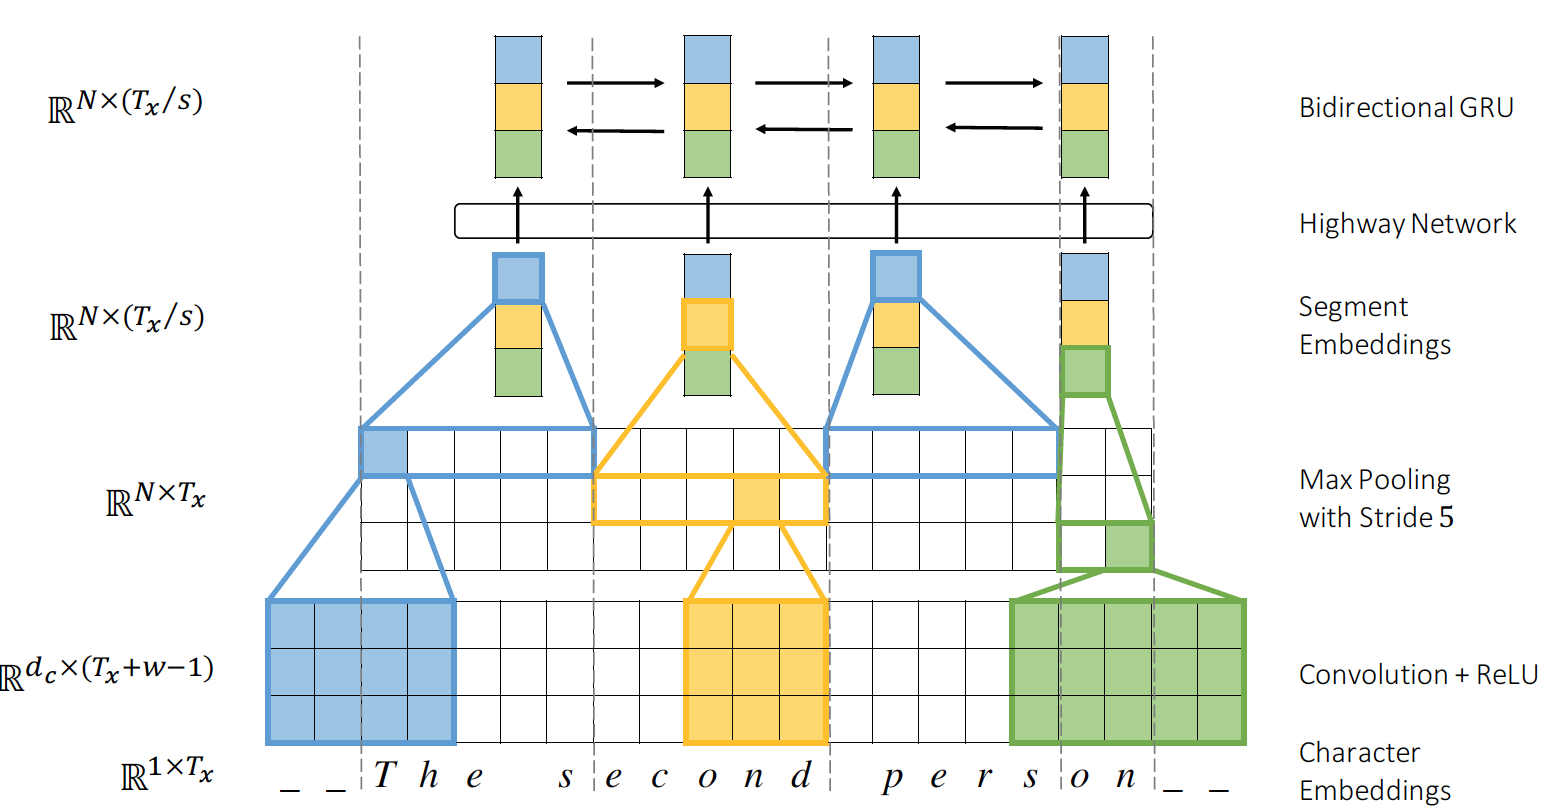
\includegraphics[width=\textwidth]{character}

\end{frame}



\section{
%%%%%%%%%%%%%%%%%%%%
%%%%%%%%%%%%%%%%%%%%
Recursive Models
%%%%%%%%%%%%%%%%%%%%
%%%%%%%%%%%%%%%%%%%%
}
\frame{\sectionpage}


%%%%%%%%%%
\begin{frame}
\frametitle{
%%%%%%%%%%
Recursive DNNs
%%%%%%%%%%
}

Make use of existing \textblue{syntactic parsers} (e.g.~constituent parsers).\\[2mm]
Parse tree defines a binary tree $\Longrightarrow$  use tree structure to compute embeddings (Socher et al, 2013)\\[4mm]

Learn composition function $g: \Re^d \times \Re^d \to \Re^d$, which is then applied at each inner node of the parse tree. \\[7mm]

\begin{columns}
\begin{column}{0.45\textwidth}
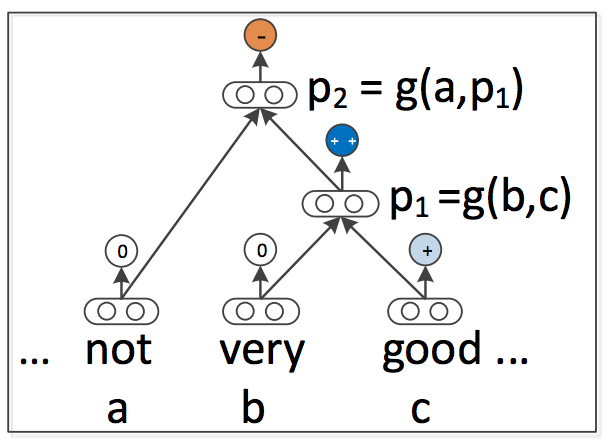
\includegraphics[width=0.99\textwidth]{recursive}
\end{column}
\begin{column}{0.45\textwidth}
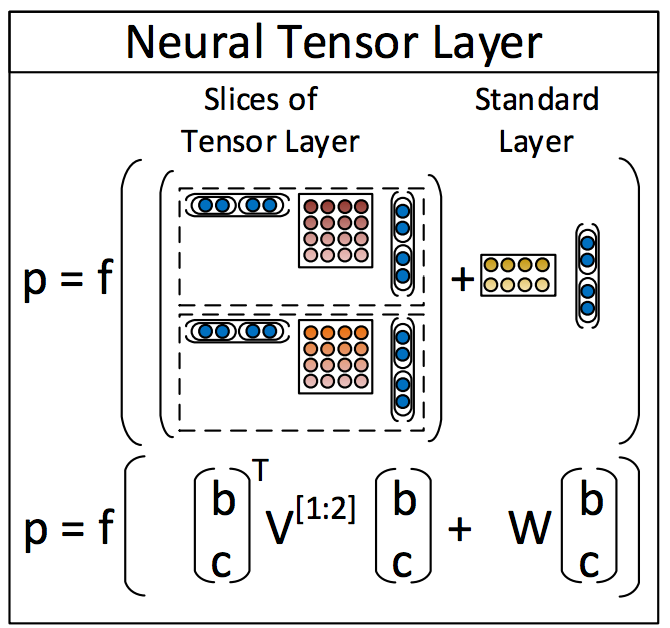
\includegraphics[width=0.8\textwidth]{tensor}
\end{column}
\end{columns}

\end{frame}

\section{
%%%%%%%%%%%%%%%%%%%%
%%%%%%%%%%%%%%%%%%%%
Conclusion
%%%%%%%%%%%%%%%%%%%%
%%%%%%%%%%%%%%%%%%%%
}
\frame{\sectionpage}



\end{document}







\section{
%%%%%%%%%%%%%%%%%%%%
%%%%%%%%%%%%%%%%%%%%
Models for Documents 
%%%%%%%%%%%%%%%%%%%%
%%%%%%%%%%%%%%%%%%%%
}
\frame{\sectionpage}

%%%%%%%%%%
\begin{frame}
\frametitle{
%%%%%%%%%%
Document Model
%%%%%%%%%%
}

\textblue{Document model}: probability distribution over text documents
\vspace*{-4mm}
\begin{center}
Document = \\
sequence of words, simplified to multiset of words 
\end{center} 
\vspace*{2mm}

Data = document collection $\D$ over vocabulary $\V = \{w_1,\dots, w_M\}$
\begin{align*}
\D = \{d_1,\dots,d_N\} , \;\;\D \ni d = (\w1,\dots, \w{L}), \;\; \w{t} \in \V 
\end{align*}
\vspace*{-5mm}

Bag-of-words assumptions = \textblue{exchangability} of word order
\begin{align*}
p(\w 1,\dots,\w L) = p(\w{\pi(1)}, \dots, \w{\pi(L)}) \;\; \text{for any $\pi \in S_L$}
\end{align*}
\vspace*{-6mm}
\begin{itemize}
\is{2mm}
\item practical plausibility; simpler mathematical treatment
\item sufficient statistics: word frequencies 
\end{itemize}

\end{frame}

%%%%%%%%%%
\begin{frame}
\frametitle{
%%%%%%%%%%
Topic Model: Single Document
%%%%%%%%%%
}

Classical model to understand \textblue{aboutness} of documents = \textred{topics}\\[4mm]

Introduce \textblue{latent topic variables}
\begin{itemize}
\is{2mm}
\item one variable $\z t$ for each observed word occurrence
\item sample space: $\z t \in [1:K]$ of $K$ topics 
\item complete data model
\vspace*{-3mm}
\begin{align*}
& d^z = ( (\w1,\z1), \dots, (\w L, \z L)), \quad 
p(d^z) = \prod_{t=1}^L p(\w t |\z t) p(\z t)
\end{align*}
\item defines a mixture model
\begin{align*}
p(d) = \sum_{(\z1,\dots,\z L)} p(d^z) = \prod_{t=1}^L \sum_{z=1}^K p(z) p(\w{t}|z)
\end{align*}
%\item parameterization
%\begin{align*}
%\beta_{ik} = p(w_i | z_k), \quad \theta_k = p(z_k)
%\end{align*}
\end{itemize} 

\end{frame}


%%%%%%%%%%
\begin{frame}
\frametitle{
%%%%%%%%%%
Topic Model: Latent Dirichlet Allocation
%%%%%%%%%%
}

Parameterization (pLSA) 
\begin{align*}
p(z)  = \theta_{zd}, & \; \; \text{document specific} \\
p(w_i|z) = \beta_{iz}, & \;\; \text{shared collection parameters}
\end{align*}

Priors (LDA)
\begin{align*}
\theta \sim \text{Dirichlet}(\alpha), \quad L \sim \text{Poisson}(\lambda)
\end{align*}

Generative model (given $\theta$, $L$ as above)
\begin{align*}
& z^t \sim \text{Multi}(\theta) \;\; (t=1,\dots,L) \\
& w^t \sim \text{Multi}(\beta_{\cdot z^t})\;\; (t=1,\dots,L)
\end{align*}

\end{frame}


\end{document}

Break-up into overlapping context windows of size $2c+1$:
\begin{align*}
(w_1,\dots,w_{2c+1}), (w_2,\dots,w_{2c+2}), \dots, (w_{T-2c},\dots,w_T)
\end{align*}


